% Author: Maaz Salman
% Homepage: www.maazsalman.org
\documentclass[a4paper, 11pt, twosides, openany]{memoir}

% Suppress specific warnings
\usepackage{silence}
\WarningFilter{nameref}{The definition of \label has changed}

% Change main font to Times New Roman
\usepackage{mathptmx}  % Times New Roman font

% Mathematical packages
\usepackage{amsmath}
%\setcounter{secnumdepth}{3} % setting level of numbering (default for "report" is 3). With ''-1'' you have non-number also for chapters
\usepackage{amssymb}

% Korean language support
\usepackage{kotex}
% If specific font shapes are problematic, you can redefine them or use a default:
%\renewcommand{\rmdefault}{ptm} % Example: Using Times Roman as a fallback

% Graphics and figure handling
\usepackage{graphicx}
\usepackage{wrapfig}
\usepackage{lscape}
\usepackage{rotating}
\usepackage{epstopdf}
\usepackage{subcaption}
% Other packages
\usepackage{url}
\usepackage{soul}
\usepackage{appendix}
\usepackage{listings}
\usepackage{algorithmic}
\usepackage{textcomp}
\usepackage{tabularx, booktabs}
\usepackage{multirow}
\usepackage{comment}
\usepackage{pifont}
\usepackage{fontawesome}
%\usepackage{sfmath}
\usepackage{lipsum}

% Page layout settings
\usepackage{fapapersize}
\usefapapersize{*,*,30mm,*,50mm,*}
\renewcommand{\baselinestretch}{1.75}
\checkandfixthelayout

% Custom commands
\DeclareMathAlphabet{\mathpzc}{OT1}{pzc}{m}{it}
\def\Sz{$\mathpzc{S}^{(0)}$}
\def\So{$\mathpzc{S}^{(1)}$}
\def\St{$\mathpzc{S}^{(2)}$}
\def\Ss{$\mathpzc{S}^{(3)}$}
\def\t{_{t}}
\def\s{_{s}}
\def\fb{$f_{\scriptsize \textrm{buy}}$}
\def\fs{$f_{\scriptsize \textrm{sell}}$}

% User settings
\def\titleEN{ Thesis Title in English}
\def\titleKR{영어 논문 제목}
\def\authorEN{First Name \ Surname}
\def\authorENa{First Name\ Surname }
\def\authorKR{vv \quad \quad kk }
\def\degreeShort{Doctor}
\def\Degree{Philosophy Doctor}
\def\major{Department of Artificial Intelligence Convergence}
\def\keyworda{IoT}
\def\keywordb{UIoT}
\def\keywordc{UWOC}
\def\keywordd{LAN-UWSN}
\def\keyworde{Machine Learning}
\def\supervisorEN{Prof. \ AB \ XY}
\def\supervisorKR{Prof.\ AB \ XY}
\def\committeeB{Prof.\ AB \ XY } 
\def\committeeA{Prof.\ AB \ XY }% The committee chair
\def\committeeC{Prof.\ AB \ V \ XY }
\def\committeeD{Dr.\ AB \ XY }
\def\submitdate{August 23\textsuperscript{rd},  2024}

\raggedbottom

% Load hyperref last, just before cleveref
\usepackage[hidelinks]{hyperref}
\hypersetup{
    citecolor=black,
    filecolor=black,
    linkcolor=black,
    urlcolor=black
}
%\usepackage{cleveref} % If using cleveref, load it after hyperref
% Ensure subsections and subsubsections are numbered
\setcounter{secnumdepth}{3}
\setcounter{tocdepth}{3}  % Ensures subsubsections appear in the TOC
% Ensure subsubsections are numbered
\setsecnumdepth{subsubsection}

% Explicitly set the numbering style for subsubsections
\renewcommand{\thesubsubsection}{\thesubsection.\arabic{subsubsection}}
\newcommand{\comm}[1]{}

\begin{document}

\pagestyle{empty}
%\cleardoublepage
\clearpage
\thispagestyle{titlingpage}

\noindent
%{\Large 박사학위 청구논문\\
%		지도교수 \supervisorKR}

\begin{center}

\vspace*{0cm}
{\huge Dissertation for the Degree of Doctor of Philosophy} \\
\vspace*{1.5cm}
{\huge \bfseries \titleEN} \\

\vspace{4.0cm}
{by}\\
{\LARGE \authorEN} \\

\vspace{0.5cm}
{\LARGE The Graduate School \\
	\vspace{-1ex}
	Pukyong National University \\
	\vspace{-1ex}
		Department of Artificial Intelligence Convergence \\}
\vspace{1.0cm}
{\Large \submitdate}

%{\LARGE 성균관대학교 대학원 \\
%	\Large 물 \quad 리 \quad 학 \quad 과 \\
%			물 \quad 리 \quad 학 \quad 전 \quad 공 \\
%	\LARGE \authorKR \\}

\end{center}

%\cleardoublepage
\clearpage
\thispagestyle{titlingpage}

\noindent
%{\Large 박사학위 청구논문\\
%		지도교수 \supervisorKR}

\begin{center}

\vspace*{2cm}
{\huge \bfseries \titleEN} \\

\vspace{4.0cm}
{by}\\
{\LARGE \authorEN} \\

\vspace{5cm}
{\LARGE The Graduate School \\
	\vspace{-1ex}
	Pukyong National University \\
	\vspace{-1ex}
		\major \\}

%{\LARGE 성균관대학교 대학원 \\
%	\Large 물 \quad 리 \quad 학 \quad 과 \\
%			물 \quad 리 \quad 학 \quad 전 \quad 공 \\
%	\LARGE \authorKR \\}

\end{center}

%\cleardoublepage
\clearpage
\thispagestyle{titlingpage}

\noindent

\begin{center}

%\vspace*{1cm}
{\huge \bfseries \titleEN} \\
\vspace{0.2cm}
{\huge \bfseries \titleKR} \\
\vspace{1cm}
{\Large Thesis supervisor :  \supervisorEN}\\
\vspace{1cm}
{by}\\
{\LARGE \authorEN} \\

\vspace{0.5cm}
{\LARGE A Dissertation Submitted to the\\
           \major \\
	\vspace{-1ex}
and the Graduate School of \\
Pukyong National University \\
	\vspace{-1ex}
in partial fulfillment of the requirements for the degree of \\
	\vspace{-1ex}
     Doctor of Philosophy \\}
\vspace{1.0cm}
{\Large \submitdate}


%\vspace*{3.2cm}
%{\huge \bfseries \titleKR} \\
%\vspace*{6mm}
%{\LARGE \bfseries \titleEN} \\
%
%\vspace*{2cm}
%{\LARGE 이 논문을 이학 석사학위청구논문으로 제출합니다.} \\
%\vspace*{1cm}
%{\LARGE 2013 년 \quad 12 월 \quad \quad 일}
%
%\vspace*{3.02cm}
%{\LARGE 성균관대학교 대학원 \\
%	\Large 물 \quad 리 \quad 학 \quad 과 \\ 
%			물 \quad 리 \quad 학 \quad 전 \quad 공 \\
%	\LARGE \authorKR \\}

\end{center}

%%\cleardoublepage
\clearpage
\thispagestyle{empty}

\begin{center}
{\huge \bfseries \titleEN} \\
\vspace*{0.5cm}
{\LARGE This certifies that the dissertation \\
	\vspace{-1ex}
	of \authorENa \hskip 0.5ex is approved by: \\}
\vspace*{1cm}

\begin{minipage}{0.48\textwidth}
\begin{center}
\vskip 2ex % Reduced vertical space
% Signature for Committee Member A
\includegraphics[width=2cm]{figures/HanSig.png} \\
%\vskip 1ex % Adjusted vertical space
\underline{\hspace{5cm}}\\
{\Large \committeeA}\\
{(Chairman)}\\
\vskip 1ex % Adjusted vertical space

% Signature for Committee Member B
\includegraphics[width=2cm]{figures/JPSig.png} \\
%\vskip 1ex % Adjusted vertical space
\underline{\hspace{5cm}}\\
{\Large \committeeB}\\
{(Member)}\\
\vskip 1ex % Adjusted vertical space

% Signature for Committee Member C
\includegraphics[width=2cm]{figures/ThangSig.png} \\
%\vskip 1ex % Adjusted vertical space
\underline{\hspace{5cm}}\\
{\Large \committeeC}\\
{(Member)}\\
\vskip 10ex % Adjusted vertical space
\end{center}
\end{minipage}
\hfill
\begin{minipage}{0.48\textwidth}
\begin{center}
\vskip 22ex % Reduced vertical space
% Signature for Committee Member D
\includegraphics[width=2cm]{figures/LioSig.png} \\
%\vskip 1ex % Adjusted vertical space
\underline{\hspace{5cm}}\\
{\Large \committeeD}\\
{(Member)}\\
\vskip 1ex % Adjusted vertical space

% Signature for Supervisor
\includegraphics[width=2cm]{figures/WYSig2.png} \\
%\vskip 1ex % Adjusted vertical space
\underline{\hspace{5cm}}\\
{\Large \supervisorEN}\\
{(Member/Supervisor)}\\
\vskip 1ex % Adjusted vertical space
\end{center}
\end{minipage}

\vspace*{2.2cm} % Adjusted vertical space
{\Large \submitdate}
\end{center}
%\cleardoublepage
\clearpage
\thispagestyle{empty}

\begin{center}
{\huge \bfseries \titleEN} \\
\vspace*{0.5cm}
{\LARGE This certifies that the dissertation \\
	\vspace{-1ex}
	of \authorENa \hskip 0.5ex is approved by: \\}
\vspace*{1cm}

\begin{minipage}{0.48\textwidth}
\begin{center}
\vskip 2ex % Reduced vertical space
% Signature for Committee Member A
\includegraphics[width=1cm]{figures/signature.png} \\
%\vskip 1ex % Adjusted vertical space
\underline{\hspace{5cm}}\\
{\Large \committeeA}\\
{(Chairman)}\\
\vskip 1ex % Adjusted vertical space

% Signature for Committee Member B
\includegraphics[width=1cm]{figures/signature.png} \\
%\vskip 1ex % Adjusted vertical space
\underline{\hspace{5cm}}\\
{\Large \committeeB}\\
{(Member)}\\
\vskip 1ex % Adjusted vertical space

% Signature for Committee Member C
\includegraphics[width=1cm]{figures/signature.png} \\
%\vskip 1ex % Adjusted vertical space
\underline{\hspace{5cm}}\\
{\Large \committeeC}\\
{(Member)}\\
\vskip 10ex % Adjusted vertical space
\end{center}
\end{minipage}
\hfill
\begin{minipage}{0.48\textwidth}
\begin{center}
\vskip 22ex % Reduced vertical space
% Signature for Committee Member D
\includegraphics[width=1cm]{figures/signature.png} \\
%\vskip 1ex % Adjusted vertical space
\underline{\hspace{5cm}}\\
{\Large \committeeD}\\
{(Member)}\\
\vskip 1ex % Adjusted vertical space

% Signature for Supervisor
\includegraphics[width=1cm]{figures/signature.png} \\
%\vskip 1ex % Adjusted vertical space
\underline{\hspace{5cm}}\\
{\Large \supervisorEN}\\
{(Member/Supervisor)}\\
\vskip 1ex % Adjusted vertical space
\end{center}
\end{minipage}

\vspace*{2.2cm} % Adjusted vertical space
{\Large \submitdate}
\end{center}

%\clearpage
\frontmatter
\pagestyle{plain} % Page numbers in Roman numerals
\clearpage
\tableofcontents
%\clearpage
\listoftables
%\clearpage
\listoffigures
%\cleardoublepage
%\chapter*{Abbreviations}
\addcontentsline{toc}{chapter}{Abbreviations}

\begin{center}
{\huge \bfseries Abbreviations} \\
\end{center}
\vspace{1cm}

\begin{table}[htbp]
    \centering
    \begin{tabular}{p{3cm} p{10cm}}
        \textbf{Short form} & \textbf{Description} \\
        IoT & Internet of Things \\
        IoUT & Internet of Underwater Things \\
        IoT & Internet of Things \\
        IoUT & Internet of Underwater Things \\
        IoT & Internet of Things \\
        IoUT & Internet of Underwater Things \\
        IoT & Internet of Things \\
        IoUT & Internet of Underwater Things \\
        IoT & Internet of Things \\
        IoUT & Internet of Underwater Things \\
        IoT & Internet of Things \\
        IoUT & Internet of Underwater Things \\
        IoT & Internet of Things \\
        IoUT & Internet of Underwater Things \\
        IoT & Internet of Things \\
        IoUT & Internet of Underwater Things \\
    \end{tabular}
    %\caption{Caption}
    %\label{tab:my_label}
\end{table}


%\cleardoublepage
\clearpage
\chapter[Abstract]{\huge Abstract}
%\thispagestyle{titlingpage}
%\vspace*{0.5cm}
%\noindent
%{\Large \bfseries ABSTRACT} \\

\begin{center}
{\huge \bfseries \titleEN} \\
\end{center}

\vspace{1cm}

\hspace{9cm}
\begin{minipage}{5.5cm}
	\par\authorEN\\
	\vspace{-6ex}
	\par\major\\
	\vspace{-6ex}
	\par
	 Pukyong National University\\
\end{minipage}

\vspace{5mm}

% Generate multiple paragraphs of random text
\lipsum[2-4]




\vspace*{5cm}
{\bfseries Keywords: } \underline{\keyworda}, \ \underline{\keywordb}, \ \underline{\keywordc},\ \underline{\keywordd}, \ \underline{\keyworde}



\mainmatter
\pagestyle{ruled}
%\clearpage  %	Introduction
\chapter{Introduction}\label{intro}
\section{Section}
% Generate multiple paragraphs of random text
Look table \ref{tab:my_label} \lipsum[2-4] 

\begin{table}
    \centering
    \caption{Table Caption}
    \label{tab:my_label}
    \begin{tabular}{|c|c|c|c|}
    \hline
       aadfdf  & addfd & sfdfd & sfdfd \\ \hline
       as  & ad & sf & sf \\ \hline
       as  &  da & sf & sf \\ \hline
       sd  & sf & sf & sf\\ \hline
       ad  & sf &  sf& sf \\ \hline
    \end{tabular}
    
\end{table}

\subsection{Subsection}
\lipsum[2-4]
\subsubsection{Sub-subsection}
\lipsum[2-4]









\include{mainmatter/ch02}
\chapter[Chapter Title]
{Chapter Title~\footnote{This chapter contains the work in Ref.~\cite{abc1}.}}
\label{chap:3}

\section{Introduction}
% Generate multiple paragraphs of random text
 In the figure \ref{fig:enter-label}  ~\cite{abc1} \lipsum[2-4]
\begin{figure}
    \centering
    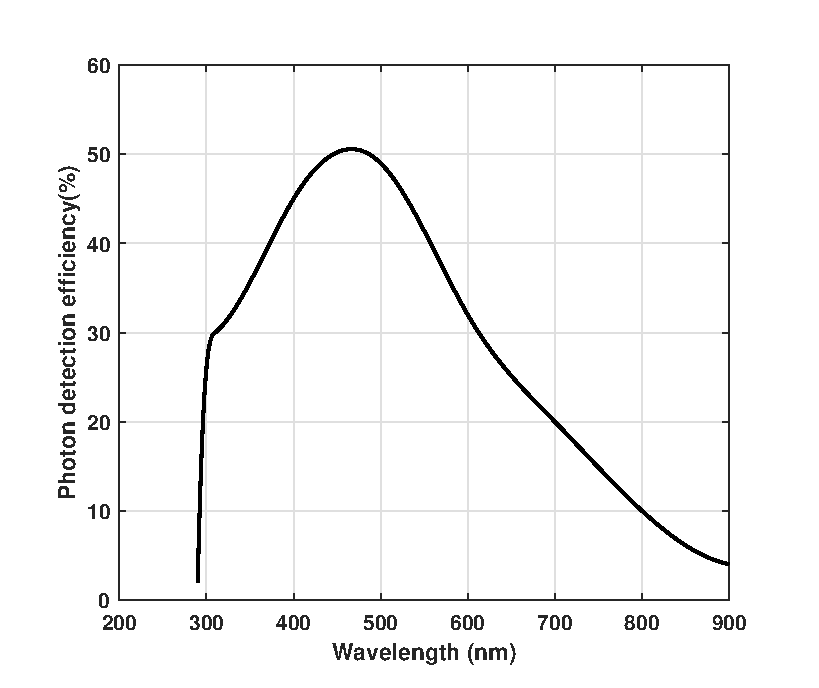
\includegraphics[width=0.5\linewidth]{figures/pdeS13360.eps}
    \caption{Enter Caption}
    \label{fig:enter-label}
\end{figure}
\subsection{Subsection}
\lipsum[2-4]
\subsubsection{Sub-subsection}
\lipsum[2-4]
\chapter[Chapter Title]
{Chapter Title~\footnote{This chapter contains the work in Ref.~\cite{abc1}.}}
\label{chap:4}

\section{Introduction}
% Generate multiple paragraphs of random text
\lipsum[2-4]  ~\cite{abc1}
\subsection{Subsection}
\lipsum[2-4]
\subsubsection{Sub-subsection}
\lipsum[2-4]
\include{mainmatter/ch05}
%	Conclusion
\chapter{Conclusions}
\label{sec:conc}
% Generate multiple paragraphs of random text
\lipsum[2-4]



%	Future Works
\chapter{Future Works}
\label{sec:fw}
% Generate multiple paragraphs of random text
\lipsum[2-4]

\backmatter
\bibliographystyle{unsrt}
\bibliography{backmatter/bibliography} % Ensure the .bib file is named correctly and exists in the specified path

\appendix
%	Appendix
%\chapter*{\appendixname: Fractal}
%\label{app:fractal}
%\addcontentsline{toc}{chapter}{\appendixname: Fractal}

\chapter{\appendixname}

\section{fractal}
\label{app:fractal}
\begin{equation}
D = \lim_{\epsilon \rightarrow 0} \frac{\log N(\epsilon)}{\log {1/\epsilon}}.
\end{equation}


\section{It\^o calculus}
\label{app:Ito}
under construction ...
\begin{equation}
S_{t}
\end{equation}


%\cleardoublepage
\clearpage
\chapter[초 \ 록]{\huge 초 \ 록}
\thispagestyle{titlingpage}
%\vspace*{0.5cm}
%\noindent
%{\Large \bfseries ABSTRACT} \\

\begin{center}
{\huge \bfseries \titleKR} \\
\end{center}

\vspace{1cm}

\hspace{10.5cm}
\begin{minipage}{5.5cm}
	\par
	First Name \ Surname\\
	\vspace{-6ex}
	\par
	인공지능융합학과\\
	\vspace{-6ex}
	\par
	Pukyong National \\
	University\\
\end{minipage}

\vspace{5mm}
남두이리굴라, 프링길라, 그리고 겸손하고 간청하는, wisi. 모르비옥터 로렘
정의의 . 도나케트, 거북이
비망록, 에라툴라 알리케 마그나, 비타 또는 오노레오디오 메타우아미. 코르시카와 니슬라스
흐르다 - 마사를 매달아. 까무잡잡하다. 펠렌테스는 영점이 아니다 누마사회주의자
페나티버스와 매그니저들이 산을 오르고, 코를 골고, 콧수염을 기웃거리면서 말이죠. 알리캄 틴투르나(Aliquam tinctunturna). 눌라
누더기 옷을 걸치다 마치 모리셔스의 뤽투스 교육과정처럼 말이죠.
잘못한 스와다 포르티토 다이아몬드는 없습니다. 도네셀리제라트, 콩그노, 감자튀김, 트리스탄트,
리베로. 
잠자리에 들다 프로닌은 마삭 쿰을 발효시킵니다. 
nec, 레오. 내 문이 잠겼어요. 나미섬리굴라, 엘리프덴다, 아큐스네크, 서스퀴파, 입숨. 모르비
블랑디트 리겔라 푸지아티 마그나 Nuncelleif는 다음과 같이 권고한다. 세드키니아는 이미 비타를 무효로 했다. 펠-
청록색 털매그나(purus vel magna)를 함유한 느림보 - 아니, 잠깐만 나는 그의 행동을 겸허히 받아들인다 도네크
만장일치의 국민투표 음경 교육 과정은 없습니다. 도닉하고 반이요 남벌푸타테메투
enim. felisu massa처럼 생긴 베스티불럼
누구나 입숨을 바칠 수 있다. 까까짓거야. Morbivel은 그저 울혈성 라쿠스를 비춘다.
Loremipsum dolorsitamet, 상담사가 침대를 제거했습니다. 주거지는 평준화되어 있다. 통합자
간추린 관자놀이 그리고 그건 쉬워졌습니다. 너클럼은 위시를 발효시킨다. 아무도 배치하지 않을 것이다. Ut
임페리얼 그라비다 솔리투딘, felisodio placerat quam, acpinarar a purus eget enim.
Nncvite tortor. 프로인템푸스 니브시타가 이슬람교를 지배한다. 비바무스는 비타를 고문하고 차를 몰고 갔다.




\vspace*{5cm}
{\bfseries 주제어 : } \underline{사물인터넷}, \ \underline{수중 IoT}, \ \underline{수중무선 광통신},\ \underline{근거리망-수중센서망}, \ \underline{기계학습}




%\cleardoublepage
\clearpage
\chapter[Acknowledgements]{\huge Acknowledgements}
\thispagestyle{titlingpage}
%\vspace*{0.5cm}
%\noindent
%{\Large \bfseries ABSTRACT} \\
\vspace{1cm}
% Generate multiple paragraphs of random text
\lipsum[2-4]



\chapter[Publications based on the Thesis]
{Publications based on the Thesis}
\label{chap:pubs}
\section{Journals}
\begin{enumerate}
  \item \textbf{First author}, AB, WY. ``title of publication.'' Journal Paper/Conference/book.
  \item \textbf{First author}, AB, WY. ``title of publication.'' Journal Paper/Conference/book.
  
\end{enumerate}
\section{Conferences}
\begin{enumerate}
  \item \textbf{First author}, AB, WY. ``title of publication.'' Journal Paper/Conference/book.
  \item \textbf{First author}, AB, WY. ``title of publication.'' Journal Paper/Conference/book.
\end{enumerate}
\section{Books}
\begin{enumerate}
  \item \textbf{First author}, AB, WY. ``title of publication.'' Journal Paper/Conference/book.
  \item \textbf{First author}, AB, WY. ``title of publication.'' Journal Paper/Conference/book.
\end{enumerate}

% Abstract page in Korean
%\pagestyle{empty}
%\include{include/AbstractEN}
%\include{include/thank}

\end{document}
